% mainfile: ../../../../master.tex
\subsection{DNA and RNA quantification with NanoDrop\cR ND-1000 Spectrophotometer}
% The part of the label after the colon must match the file name. Otherwise,
% conditional compilation based on task labels does NOT work.
\label{task:20180215_cj0}
\tags{lab,qnt,dna,rna}
\authors{cj}
%\files{}
%\persons{}

Today, I want to quantify the DNA and RNA concentration obtained from 4~mL of micro-algae cultures with the MasterPure\texttrademark~ kit.

\begin{figure}[H] % position of the figure 
    \centering
    \caption{Spectra of the DNA and the RNA extracted from micro-algae cultures with the Modified MasterPure\texttrademark~ method}
    \label{fig:CJ20180215_DNA_RNA_MasterPure}
    \begin{subfigure}[b]{0.49\textwidth}
        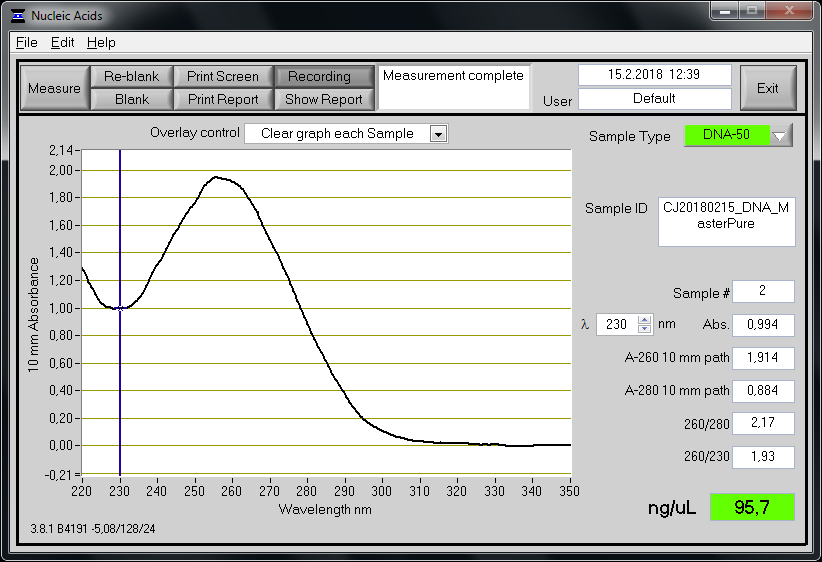
\includegraphics[width=\textwidth]{graphics/screenshots/CJ20180215_DNA_MasterPure.png}
        \caption{DNA}
        \label{sfig:CJ20180215_DNA_MasterPure}
    \end{subfigure}
    ~ 
    \begin{subfigure}[b]{0.49\textwidth}
        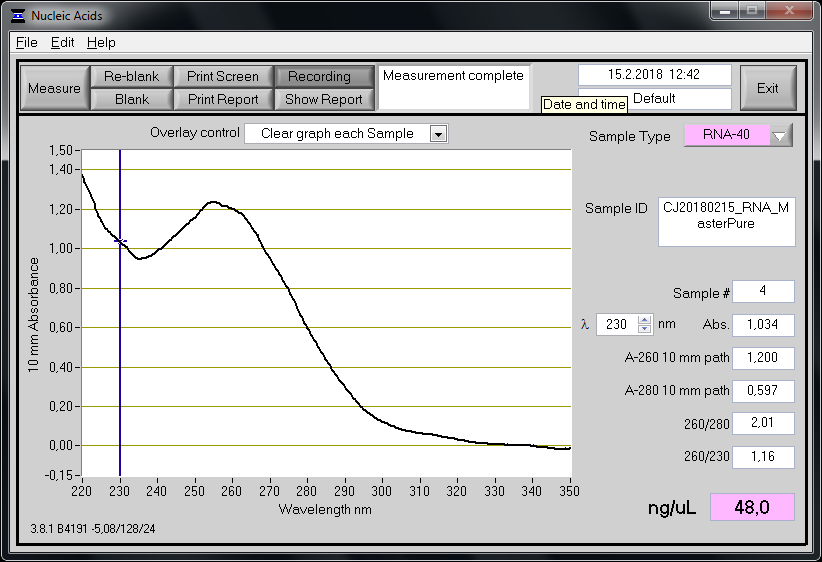
\includegraphics[width=\textwidth]{graphics/screenshots/CJ20180215_RNA_MasterPure.png}
        \caption{RNA}
        \label{sfig:CJ20180215_RNA_MasterPure}
    \end{subfigure}
\end{figure}

\comment{I made sure the blanks are close to the baseline because it seems that last time something went wrong with the blank which lead to weird ratios.}

\begin{table}[htbp]
\caption{res/nanodrop/CJ20180215.txt}
\label{tab:CJ20180215}
\centering
\begin{tabular}{l l l l l l l l l l l l l }
\toprule
Sample ID & Time  & ng/ul  & A260  & A280  & 260/280  & 260/230  \\ \midrule
\texttt{CJ20180215\_BLANK} & 12:38 & -0.01 & -0,000 & -0,001 & 0,42 & -0,02 \\
\texttt{CJ20180215\_DNA\_MasterPure} & 12:39 & 95,71 & 1,914 & 0,884 & 2,17 & 1,93 \\
\texttt{CJ20180215\_BLANK} & 12:41 & 0,12 & 0,003 & -0,011 & -0,27 & 0,17 \\
\texttt{CJ20180215\_RNA\_MasterPure} & 12:42 & 47,99 & 1,200 & 0,597 & 2,01 & 1,16 \\
\bottomrule
\end{tabular}
\end{table}

The absorbance measurments are shown in table \ref{tab:CJ20180215}. The 260/280 ratio measured for the DNA is 2.17 which is higher than the expected value of 1.8. But I am not worried about that because a high 260/280 purity ratio is not indicative of an issue (it is very likely due to the slightly alkaline pH of the Tris HCl which is known over-represent the ratio by 0.2–0.3). The 260/230 ratio measured for the RNA is 1.93 which is pretty good, but still a little lower than the expected values that are supposed to be between 2.0 and 2.2. This slightly low 260/230 ratio could be explained by the presence of contaminants absorbing at 230 nm such as \gls{edta}, carbohydrates, phenol, glycogen, or guanidine HCl. In this case, it cannot be phenol because I know there are not phenol involved in the MasterPure\texttrademark~ method. My guess is that this slightly low 260/230 ratio may be the resul of carbohydrate carryover which is known to be a problem with plants, and therefore - I suspect - with micro-algae.

The 260/280 ratio measured for the RNA is 2.01 which is the expected value! However, concerning the 260/230 ratio, it is a little lower than the expected values, which can be explained in the same way as it is for the 260/230 ratio measured for the DNA.

But overall, the spectra look a lot better than any I have obtained so far when extracting DNA and RNA from a single sample.